\chapter{Chapter 4: Weyl tensor and gravitational radiation}
In this chapter we return to the linearized gravitational field, but in this case we want to obtain an expression that depends of the origin of curvature which contributes to the linearized gravitational field. For this the tetrad concept is introduce, together with the Newman-Penrose formalism and the Weyl scalars. The final flux equations are obtained in terms of a particular Weyl scalar, which is the geometric origin of curvature. Main references for this chapter are \cite{Chandrasekhar,Alcubierre,Ruiz}
\section{Tetrads and Newman-Penrose formalism}
\subsection{Tetrads}

Here we are going to define four linearly independent vectors on a
local coordinate system as basis and name some properties of this
vectors. We set up at each point of space-time a basis of four vectors
\[
\boldsymbol{e}_{(a)}=e_{(a)}^{\alpha}\partial_{\alpha},
\]
where $a=0,1,2,3$. This vectors are known as \textbf{tetrad basis},
the enclosure in parentheses distinguishes the tetrad indices from
the tensor indices. Just like any other vector we have that
\[
e_{(a)\alpha}=g_{\alpha\beta}e_{(a)}^{\beta}.
\]
To define its inverse we have the following relations
\[
e_{(a)}^{\alpha}e_{\alpha}^{(b)}=\delta_{(a)}^{(b)},\hspace{1em}e_{(a)}^{\alpha}e_{\beta}^{(a)}=\delta_{\beta}^{\alpha},
\]
and we will also assume that
\[
e_{(a)}^{\alpha}e_{(b)\alpha}=\eta_{(a)(b)}
\]
where $\eta_{(a)(b)}$ is constant and symmetric. 
\begin{figure}[h]
\centering{}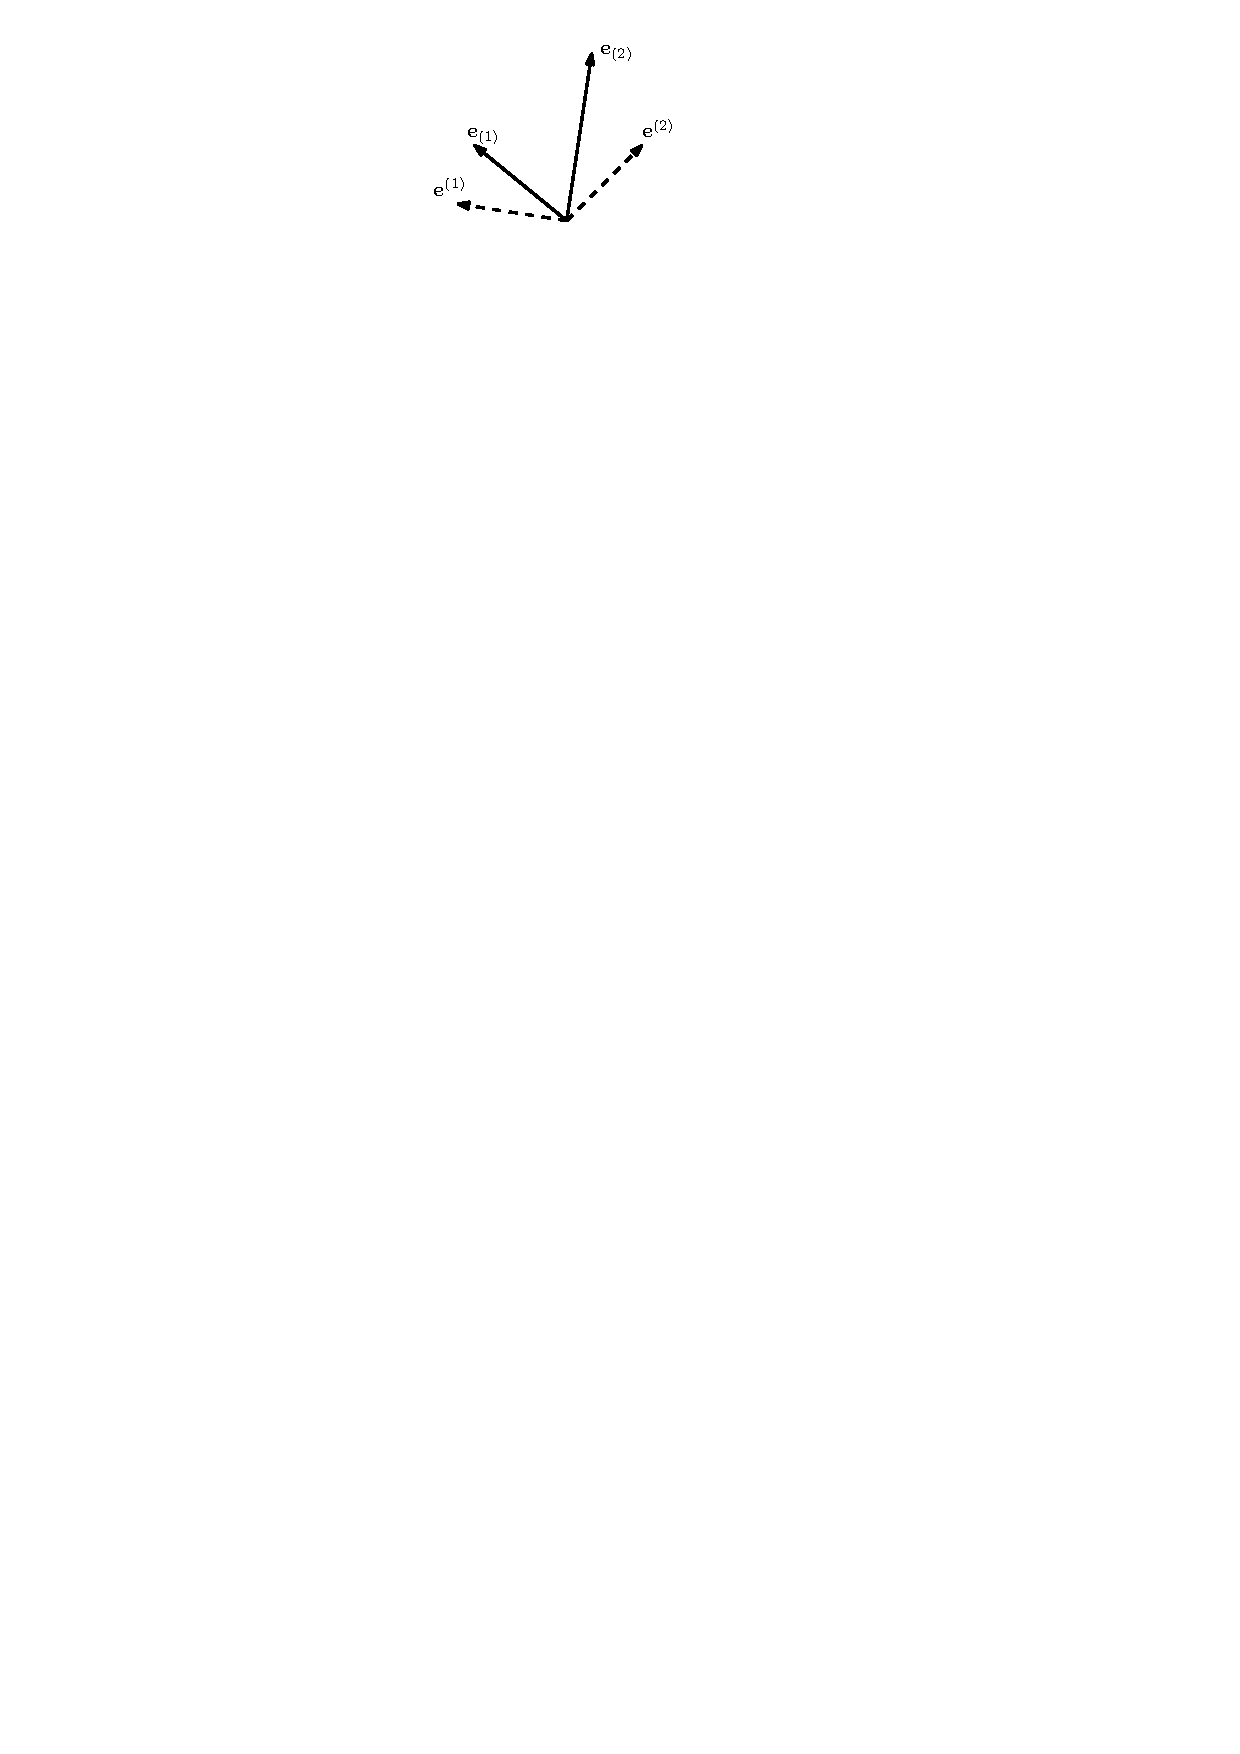
\includegraphics[scale=1.1]{Kap5/tetrads.pdf}\caption{Starting from the two vectors $\left(\boldsymbol{e}_{(1)},\boldsymbol{e}_{(2)}\right)$,
we construct a new vectors $\left(\boldsymbol{e}^{(1)},\boldsymbol{e}^{(2)}\right)$
such that $\boldsymbol{e}_{(1)}\cdot\boldsymbol{e}^{(2)}=0$, $\boldsymbol{e}_{(2)}\cdot\boldsymbol{e}^{(1)}=0$,
$\boldsymbol{e}_{(1)}\cdot\boldsymbol{e}^{(1)}=0$ and $\boldsymbol{e}_{(2)}\cdot\boldsymbol{e}^{(2)}=0$. Traced image from \cite{Alcubierre}\label{fig:tetrads}}
\end{figure}

We will not define yet the values of $\eta_{(a)(b)}$, we will only
say that are constant. The inverse of $\eta_{(a)(b)}$ is defined
in such a way that
\[
\eta_{(a)(b)}\eta^{(b)(c)}=\delta_{(a)}^{(b)},
\]
and as a consequence of the various definitions
\begin{equation}
\eta_{(a)(b)}e_{\alpha}^{(b)}=e_{(b)\alpha},\hspace{1em}\eta^{(a)(b)}e_{(b)\alpha}=e_{\alpha}^{(a)}
\end{equation}
and
\begin{equation}
e_{(a)\alpha}e_{\beta}^{(a)}=g_{\alpha\beta}.\label{eq:g-tetrad}
\end{equation}
A graphical representation of the relation between tetrads is given
in figure \ref{fig:tetrads}.

Given any tensor field, we project it onto the tetrad frame to obtain
its tetrad components. Thus
\begin{align*}
A_{(a)}= & \ e_{(a)\alpha}A^{\alpha}=e_{(a)}^{\alpha}A_{\alpha},\\
A^{(a)}= & \ \eta^{(a)(b)}A_{(b)}=e_{\alpha}^{(a)}A^{\alpha}=e^{(a)\alpha}A_{\alpha},\\
A^{\alpha}= & \ e_{(a)}^{\alpha}A^{(a)}=e^{(a)\alpha}A_{(a)},
\end{align*}
in a more general way we have
\begin{align*}
T_{(a)(b)}= & \ e_{(a)}^{\alpha}e_{(b)}^{\beta}T_{\alpha\beta}=e_{(a)}^{\alpha}T_{\alpha(b)},\\
T_{\alpha\beta}= & \ e_{\alpha}^{(a)}e_{\beta}^{(b)}T_{(a)(b)}=e_{\alpha}^{(a)}T_{(a)\beta}.
\end{align*}

\subsection{Newman-Penrose formalism}

Here we have a special choice of basis vectors, these vectors are
a tetrad $\boldsymbol{l}$, $\boldsymbol{n}$, $\boldsymbol{m}$ and
$\boldsymbol{m}^{*}$, where $\boldsymbol{l}$ and $\boldsymbol{n}$
are real and $\boldsymbol{m}$ and $\boldsymbol{m}^{*}$ are complex
conjugates of one another. These vectors are null and they satisfy
the following orthogonality conditions
\[
\boldsymbol{l}\cdot\boldsymbol{m}=\boldsymbol{l}\cdot\boldsymbol{m}^{*}=\boldsymbol{n}\cdot\boldsymbol{m}=\boldsymbol{n}\cdot\boldsymbol{m}^{*}=0,
\]
besides the requirements
\[
\boldsymbol{l}\cdot\boldsymbol{l}=\boldsymbol{n}\cdot\boldsymbol{n}=\boldsymbol{m}\cdot\boldsymbol{m}=\boldsymbol{m}^{*}\cdot\boldsymbol{m}^{*}=0.
\]
The vectors fulfill the following normalizations conditions
\begin{align*}
\boldsymbol{l}\cdot\boldsymbol{m}= & \ 1,\\
\boldsymbol{m}\cdot\boldsymbol{m}^{*}= & \ -1.
\end{align*}
The constructed vectors are given by
\begin{align}
\boldsymbol{l} & =\frac{1}{\sqrt{2}}\left(\boldsymbol{e}_{(0)}+\boldsymbol{e}_{(1)}\right)\label{eq:tetrad-l}\\
\boldsymbol{n} & =\frac{1}{\sqrt{2}}\left(\boldsymbol{e}_{(0)}-\boldsymbol{e}_{(1)}\right)\label{eq:tetrad-n}\\
\boldsymbol{m} & =\frac{1}{\sqrt{2}}\left(\boldsymbol{e}_{(2)}+i\boldsymbol{e}_{(3)}\right)\label{eq:tetrad-m}\\
\boldsymbol{m}^{*} & =\frac{1}{\sqrt{2}}\left(\boldsymbol{e}_{(2)}-i\boldsymbol{e}_{(3)}\right)\label{eq:tetrad-m2}
\end{align}

For $\eta_{(a)(b)}$, is defined in such a way that
\[
\eta_{(a)(b)}=\eta^{(a)(b)}=\left(\begin{array}{cccc}
0 & -1 & 0 & 0\\
-1 & 0 & 0 & 0\\
0 & 0 & 0 & 1\\
0 & 0 & 1 & 0
\end{array}\right).
\]
The four vectors $\left(\boldsymbol{l},\boldsymbol{n},\boldsymbol{m},\boldsymbol{m}^{*}\right)$
form what is known as a null tetrad. Using (\ref{eq:g-tetrad})
\[
g_{\alpha\beta}=-l_{\alpha}n_{\beta}-n_{\alpha}l_{\beta}+m_{\alpha}m_{\beta}^{*}+m_{\alpha}^{*}m_{\beta}.
\]

\section{The Weyl tensor}

The Weyl tensor for a 4 dimensional manifold is defined as
\[
C_{\alpha\beta\gamma\delta}=R_{\alpha\beta\gamma\delta}-\frac{1}{2}\left(g_{\alpha\gamma}R_{\beta\delta}+g_{\beta\delta}R_{\alpha\gamma}-g_{\beta\gamma}R_{\alpha\delta}-g_{\alpha\delta}R_{\beta\gamma}\right)+\frac{1}{6}R\left(g_{\alpha\gamma}g_{\beta\delta}-g_{\beta\gamma}g_{\alpha\delta}\right).
\]
All contractions of the Weyl tensor vanish identically,
\[
C_{\beta\alpha\delta}^{\alpha}=0,
\]
while its index symmetries are identically to those of the Riemann
tensor,
\[
\begin{array}{l}
C_{\alpha\beta\gamma\delta}=-C_{\beta\alpha\gamma\delta}=C_{\alpha\beta\delta\gamma}=C_{\gamma\delta\alpha\beta},\\
C_{\alpha\beta\gamma\delta}+C_{\alpha\beta\gamma\delta}+C_{\alpha\beta\gamma\delta}=0.
\end{array}
\]
We can write it in its tetrad components
\begin{align*}
C_{(a)(b)(c)(d)}= & \ R_{(a)(b)(c)(d)}+\frac{1}{2}\left(\eta_{(a)(c)}R_{(b)(d)}-\eta_{(b)(c)}R_{(a)(d)}-\eta_{(a)(d)}R_{(b)(c)}+\eta_{(b)(d)}R_{(a)(c)}\right)\\
\  & \ +\frac{1}{6}\left(\eta_{(a)(c)}\eta_{(b)(d)}-\eta_{(a)(d)}\eta_{(b)(c)}\right),
\end{align*}
in the Newman-Penrose formalism, the ten independent components of
the Weyl tensor are represented by the five complex scalars
\begin{align}
\Psi_{0}= & \ C_{(0)(2)(0)(2)}=C_{\alpha\beta\gamma\delta}l^{\alpha}m^{\beta}l^{\gamma}m^{\delta}\\
\Psi_{1}= & \ C_{(0)(1)(0)(2)}=C_{\alpha\beta\gamma\delta}l^{\alpha}n^{\beta}l^{\gamma}m^{\delta}\\
\Psi_{2}= & \ C_{(0)(2)(3)(1)}=C_{\alpha\beta\gamma\delta}l^{\alpha}m^{\beta}m^{*\gamma}n^{\delta}\\
\Psi_{3}= & \ C_{(1)(2)(3)(2)}=C_{\alpha\beta\gamma\delta}l^{\alpha}n^{\beta}m^{*\gamma}n^{\delta}\\
\Psi_{4}= & \ C_{(1)(3)(1)(3)}=C_{\alpha\beta\gamma\delta}n^{\alpha}m^{*\beta}n^{\gamma}m^{*\delta},\label{eq:psi4}
\end{align}
this scalars are useful, in particular $\Psi_{4}$, for the radiated
energy and momentum expressions.

\subsection{Radiated energy and momentum}

Let us define the complex quantity $H$ such that
\[
H=h^{+}-ih^{\times},
\]
we can write the average
\[
\left\langle \left(\partial_{t}h^{+}\right)^{2}+\left(\partial_{t}h^{\times}\right)^{2}\right\rangle 
\]
in terms of $H$. We have that
\[
\partial_{\alpha}H\partial_{\beta}H^{*}=\left[\partial_{\alpha}h^{+}\partial_{\beta}h^{+}+\partial_{\alpha}h^{\times}\partial_{\beta}h^{\times}\right]+i\left[\partial_{\alpha}h^{+}\partial_{\beta}h^{\times}-\partial_{\alpha}h^{\times}\partial_{\beta}h^{+}\right],
\]
we take the following case
\[
\partial_{t}H\partial_{r}H^{*}=\left[\partial_{t}h^{+}\partial_{r}h^{+}+\partial_{t}h^{\times}\partial_{r}h^{\times}\right]+i\left[\partial_{t}h^{+}\partial_{r}h^{\times}-\partial_{t}h^{\times}\partial_{r}h^{+}\right],
\]
then
\begin{equation}
\text{Re}\left(\partial_{t}H\partial_{r}H^{*}\right)=\partial_{t}h^{+}\partial_{r}h^{+}+\partial_{t}h^{\times}\partial_{r}h^{\times},\label{eq:reh}
\end{equation}
where $\text{Re}\left(\cdots\right)$ is the real part of a complex
number. In the second chapter we show that $\partial_{r}h_{ij}^{TT}\left(t,r\right)\approx-\partial_{0}h_{ij}^{TT}\left(t,r\right)$
in the radiation zone, therefore
\begin{align*}
\left\langle \partial_{t}H\partial_{r}H^{*}\right\rangle = & \ \left\langle \partial_{t}H\partial_{t}H^{*}\right\rangle \\
= & \ \left\langle \left|\partial_{t}H\right|^{2}\right\rangle 
\end{align*}
and from (\ref{eq:reh})
\[
\left\langle \left|\partial_{t}H\right|^{2}\right\rangle =\left\langle \left(\partial_{t}h^{+}\right)^{2}+\left(\partial_{t}h^{\times}\right)^{2}\right\rangle .
\]
This allow us to write equation (\ref{eq:dedt-ch2}) as
\[
\frac{dE}{dt}=\frac{c^{3}r^{2}}{16\pi G}\int\left\langle \left|\partial_{t}H\right|^{2}\right\rangle d\Omega.
\]

We construct a null tetrad from the orthonormal spherical basis using
the equations (\ref{eq:tetrad-l}), (\ref{eq:tetrad-n}), (\ref{eq:tetrad-m})
and (\ref{eq:tetrad-m2})
\begin{align*}
l^{\alpha}:= & \frac{1}{\sqrt{2}}\left(e_{t}^{\alpha}+e_{r}^{\alpha}\right),\\
n^{\alpha}:= & \frac{1}{\sqrt{2}}\left(e_{t}^{\alpha}-e_{r}^{\alpha}\right),\\
m^{\alpha}:= & \frac{1}{\sqrt{2}}\left(e_{\theta}^{\alpha}+ie_{\phi}^{\alpha}\right),\\
m^{*\alpha}:= & \frac{1}{\sqrt{2}}\left(e_{\theta}^{\alpha}-ie_{\phi}^{\alpha}\right),
\end{align*}
where the vectors $\boldsymbol{e}_{t}$, $\boldsymbol{e}_{r}$,
$\boldsymbol{e}_{\theta}$ and $\boldsymbol{e}_{\phi}$ are the
usual orthonormal basis induced by the spherical coordinates. Calculating
$\Psi_{4}$ from equation (\ref{eq:psi4}) and the null tetrad constructed
above, knowing that there is no explicit dependence of $t$, $\theta$
and $\phi$ we obtain that
\[
\Psi_{4}=-\frac{1}{4}\left(\partial_{t}^{2}h^{+}-2\partial_{t}\partial_{r}h^{+}+\partial_{r}^{2}h^{+}\right)+\frac{i}{4}\left(\partial_{t}^{2}h^{\times}-2\partial_{t}\partial_{r}h^{\times}+\partial_{r}^{2}h^{\times}\right),
\]
given that we are in the local wave zone then $\partial_{r}h=-\partial_{0}h$,
therefore
\[
\Psi_{4}=-\partial_{t}^{2}h^{+}+i\partial_{t}^{2}h^{\times}=-\partial_{t}^{2}H.
\]
This implies that for outgoing gravitational waves we can write
\begin{equation}
H=-\int_{-\infty}^{t}\int_{-\infty}^{t'}\Psi_{4}dt''dt',\label{eq:h-psi4}
\end{equation}
then the total flux energy leaving the system is
\[
\frac{dE}{dt}=\frac{c^{3}r^{2}}{16\pi G}\int\left|\int_{-\infty}^{t}\Psi_{4}dt'\right|^{2}d\Omega.
\]

Now we are going to write the flux of momentum along the radial direction,
this expression is given in Chapter \ref{chp2}, writing it in term of $H$ we
have that
\[
\frac{dP_{i}}{dt}=\frac{c^{3}r^{2}}{16\pi G}\int k_i\left|\partial_{t}H\right|^{2}d\Omega
\]
where
\[
k_i=\frac{\boldsymbol{x}}{r}=\left(\sin\theta\cos\varphi,\sin\theta\sin\varphi,\cos\theta\right),
\]
for this it was used the fact that in the wave zone the angular dependence can be neglected, then $\partial_iH=\left(x_i/r\right)\partial_rH$ and that $\partial_{r}h=-\partial_{0}h$. Then, from (\ref{eq:h-psi4}) we finally got
\[
\frac{dP_{i}}{dt}=\frac{c^{3}r^{2}}{16\pi G}\int k_i\left|\int_{-\infty}^{t}\Psi_{4}dt'\right|^{2}d\Omega.
\]

Now we are going to calculate the flux of angular momentum, we are
going to calculate it from the expression (\ref{eq:an-mom-flux}). We are going
to rewrite this expression introducing the angular vectors $\boldsymbol{\xi}_{i}$
associated to rotations around the three coordinate axis. These vectors
are Killing fields of the flat metric, and in Cartesian coordinates
have components given by $\xi_{i}^{k}=\epsilon_{i}^{jk}x_{j}$\footnote{This can be view from the general solution of the Killing equation
in flat spacetime, from eq. (\ref{eq:killing-general}) we take $a_{\alpha}=0$ and
particular values for $l_{\alpha\beta}$ such that we obtain this
form of the vector.}, where $\xi_{i}^{k}$ represents the $k$ component of the vector
$\boldsymbol{\xi}_{i}$. Let us write the flux of angular momentum
in terms of the Lie derivative, for this we are going to use the expression
\begin{equation}
\left(\mathcal{L}_{\boldsymbol{\xi}_{i}}\boldsymbol{h}\right)_{\alpha\beta}=\xi_{i}^{\sigma}\partial_{\sigma}h_{\alpha\beta}+h_{\sigma\beta}\partial_{\alpha}\xi_{i}^{\sigma}+h_{\alpha\sigma}\partial_{\beta}\xi_{i}^{\sigma},\label{eq:lie-wav}
\end{equation}
given that we are in the local wave zone we restrict ourselves to
the index $a,b,c,...$ where these run from 1 to 2. If we multiply
(\ref{eq:lie-wav}) by $\partial_{r}h^{ab}$ and sum over $a$ and
$b$, because $\boldsymbol{\xi}_{i}$ is a Killing vector then
\[
h_{cb}\partial_{a}\xi_{i}^{c}\partial_{r}h^{ab}+h_{ac}\partial_{b}\xi_{i}^{c}\partial_{r}h^{ab}=0,
\]
and because we are in the gauge TT the term $\left(2\delta_{aj}\epsilon_{i}^{jk}h_{bj}\right)\partial_{r}h^{ab}=0.$
Then we can write the flux of angular momentum as
\begin{equation}
\frac{dJ_{i}}{dt}=-\frac{c^{3}r^{2}}{32\pi G}\int\left(\mathcal{L}_{\boldsymbol{\xi}_{i}}\boldsymbol{h}\right)_{ab}\partial_{r}h^{ab}d\Omega.\label{eq:djdt-lie}
\end{equation}
Now we want to write (\ref{eq:djdt-lie}) in terms of $H$, for this
we are going to introduce spherical coordinates $(r,\theta,\varphi)$,
this implies that
\begin{align*}
\boldsymbol{\xi}_{x}= & \ \left(0,-\sin\varphi,-\cos\varphi\cot\theta\right)\\
\boldsymbol{\xi}_{y}= & \ \left(0,\cos\varphi,-\sin\varphi\cot\theta\right)\\
\boldsymbol{\xi}_{z}= & \ \left(0,0,1\right),
\end{align*}
because along $\boldsymbol{\xi}_{z}$ the Lie derivatives reduce to
partial derivatives, we are going to introduce two angular vectors
to calculate the Lie derivatives in the other directions

\begin{align*}
\boldsymbol{\xi}_{\pm}= & \ \boldsymbol{\xi}_{x}\pm i\boldsymbol{\xi}_{y}\\
= & \ e^{\pm i\varphi}\left(0,\pm i,-\cot\theta\right).
\end{align*}
Let us also introduce an orthonormal spherical basis $(\boldsymbol{e}_{r},\boldsymbol{e}_{\theta},\boldsymbol{e}_{\varphi})$
and two unit complex vectors
\begin{align*}
\boldsymbol{e}_{\pm}= & \ \frac{1}{\sqrt{2}}\left(\boldsymbol{e}_{\theta}\pm i\boldsymbol{e}_{\varphi}\right)\\
= & \ \frac{1}{r\sqrt{2}}\left(0,1,\mp i\csc\theta\right).
\end{align*}

Let us calculate the Lie derivative of $\boldsymbol{e}_{\pm}$ along
$\boldsymbol{\xi}_{\pm}$, because these are vectors we calculate
the Lie derivative with the Lie brackets
\begin{align*}
\mathcal{L}_{\boldsymbol{\xi}_{\pm}}\boldsymbol{e}_{\pm}= & \ \left[\boldsymbol{\xi}_{\pm},\boldsymbol{e}_{\pm}\right]\\
= & \ \left[\pm ie^{\pm i\varphi}\partial_{\theta}-e^{\pm i\varphi}\cot\theta\partial_{\varphi}\right]\left(\frac{1}{r\sqrt{2}}\partial_{\theta}\mp\frac{i}{r\sqrt{2}}\csc\theta\right)\\
\  & \ -\left[\frac{1}{r\sqrt{2}}\partial_{\theta}\mp\frac{i}{r\sqrt{2}}\csc\theta\partial_{\varphi}\right]\left(\pm ie^{\pm i\varphi}\partial_{\theta}-e^{\pm i\varphi}\cot\theta\partial_{\varphi}\right),
\end{align*}
calculating the derivatives and factoring we have
\[
\left(\mathcal{L}_{\boldsymbol{\xi}_{\pm}}\boldsymbol{e}_{\pm}\right)^{a}=\mp\left(ie^{\pm i\varphi}\csc\theta\right)\left(\boldsymbol{e}_{\pm}\right)^{a}.
\]

Now we write the linearized field $h_{ab}$ in the TT gauge in terms
of the orthonormal basis
\begin{align*}
h_{ab}= & \ h^{+}\left[\left(\boldsymbol{e}_{\theta}\right)_{a}\left(\boldsymbol{e}_{\theta}\right)_{b}-\left(\boldsymbol{e}_{\varphi}\right)_{a}\left(\boldsymbol{e}_{\varphi}\right)_{b}\right]+h^{\times}\left[\left(\boldsymbol{e}_{\theta}\right)_{a}\left(\boldsymbol{e}_{\varphi}\right)_{b}-\left(\boldsymbol{e}_{\varphi}\right)_{a}\left(\boldsymbol{e}_{\theta}\right)_{b}\right]\\
= & \ \left(h^{+}-ih^{\times}\right)\left(\boldsymbol{e}_{-}\right)_{a}\left(\boldsymbol{e}_{-}\right)_{b}+\left(h^{+}+ih^{\times}\right)\left(\boldsymbol{e}_{+}\right)_{a}\left(\boldsymbol{e}_{+}\right)_{b}\\
= & \ H\left(\boldsymbol{e}_{-}\right)_{a}\left(\boldsymbol{e}_{-}\right)_{b}+\bar{H}\left(\boldsymbol{e}_{+}\right)_{a}\left(\boldsymbol{e}_{+}\right)_{b},
\end{align*}
with this we have
\begin{align*}
\left(\mathcal{L}_{\boldsymbol{\xi}_{\pm}}\boldsymbol{h}\right)_{ab}= & \ H\left[\left(\mathcal{L}_{\boldsymbol{\xi}_{\pm}}\boldsymbol{e}_{-}\right)_{a}\left(\boldsymbol{e}_{-}\right)_{b}+\left(\boldsymbol{e}_{-}\right)_{a}\left(\mathcal{L}_{\boldsymbol{\xi}_{\pm}}\boldsymbol{e}_{-}\right)_{b}\right]+\bar{H}\left[\left(\mathcal{L}_{\boldsymbol{\xi}_{\pm}}\boldsymbol{e}_{+}\right)_{a}\left(\boldsymbol{e}_{+}\right)_{b}+\left(\boldsymbol{e}_{+}\right)_{a}\left(\mathcal{L}_{\boldsymbol{\xi}_{\pm}}\boldsymbol{e}_{+}\right)_{b}\right]\\
= & \ -2ie^{\pm i\varphi}\csc\theta\left(\boldsymbol{e}_{-}\right)_{a}\left(\boldsymbol{e}_{-}\right)_{b}H+2ie^{\pm i\varphi}\csc\theta\left(\boldsymbol{e}_{-}\right)_{a}\left(\boldsymbol{e}_{-}\right)_{b}\bar{H}.
\end{align*}
Let us define the following operators
\[
\hat{J}_{\pm}=\xi_{\pm}^{a}\partial_{a}-ise^{\pm i\varphi}\csc\theta=e^{\pm i\varphi}\left(\pm i\partial_{\theta}-\cot\theta\partial_{\varphi}-is\csc\theta\right),
\]
where $s$ is known as the spin weight of the function\footnote{For details of the general theory where the spin weight of a function
is used see \cite{Alcubierre} Appendix D}, $s=-2$ for $H$ and $s=2$ for $\bar{H}$, then
\[
\left(\mathcal{L}_{\boldsymbol{\xi}_{\pm}}\boldsymbol{h}\right)_{ab}=\left(\boldsymbol{e}_{-}\right)_{a}\left(\boldsymbol{e}_{-}\right)_{b}\hat{J}_{\pm}H+\left(\boldsymbol{e}_{+}\right)_{a}\left(\boldsymbol{e}_{+}\right)_{b}\hat{J}_{\pm}\bar{H}.
\]
Calculating $\left(\mathcal{L}_{\boldsymbol{\xi}_{\pm}}\boldsymbol{h}\right)_{ab}\partial_{t}h^{ab}$
\begin{align*}
\left(\mathcal{L}_{\boldsymbol{\xi}_{\pm}}\boldsymbol{h}\right)_{ab}\partial_{t}h^{ab}= & \ \left[\left(\boldsymbol{e}_{-}\right)_{a}\left(\boldsymbol{e}_{-}\right)_{b}\hat{J}_{\pm}H+\left(\boldsymbol{e}_{+}\right)_{a}\left(\boldsymbol{e}_{+}\right)_{b}\hat{J}_{\pm}\bar{H}.\right]\partial_{t}\left[H\left(\boldsymbol{e}_{-}\right)_{a}\left(\boldsymbol{e}_{-}\right)_{b}+\bar{H}\left(\boldsymbol{e}_{+}\right)_{a}\left(\boldsymbol{e}_{+}\right)_{b}\right],
\end{align*}
because $\boldsymbol{e}_{\theta}$ and $\boldsymbol{e}_{\varphi}$
are orthogonal $\left(\boldsymbol{e}_{-}\right)_{a}\left(\boldsymbol{e}_{-}\right)^{a}=\left(\boldsymbol{e}_{+}\right)_{b}\left(\boldsymbol{e}_{+}\right)^{b}=0$
and $\left(\boldsymbol{e}_{-}\right)_{a}\left(\boldsymbol{e}_{+}\right)^{a}=\left(\boldsymbol{e}_{+}\right)_{b}\left(\boldsymbol{e}_{-}\right)^{b}=1$,
therefore
\begin{equation}
\left(\mathcal{L}_{\boldsymbol{\xi}_{\pm}}\boldsymbol{h}\right)_{ab}\partial_{t}h^{ab}=\hat{J}_{\pm}H\partial_{t}\bar{H}+\hat{J}_{\pm}\bar{H}\partial_{t}H=2\text{Re}\left\{ \hat{J}_{\pm}H\partial_{t}\bar{H}\right\} .\label{eq:lehj}
\end{equation}
From (\ref{eq:lehj}) and the properties of the Lie derivative
\begin{align}
\hat{J}_{+}H\partial_{t}\bar{H}+\hat{J}_{+}\bar{H}\partial_{t}H= & \ \left(\mathcal{L}_{\boldsymbol{\xi}_{x}}\boldsymbol{h}+i\mathcal{L}_{\boldsymbol{\xi}_{y}}\boldsymbol{h}\right)_{ab}\partial_{t}h_{ab}\label{eq:jh+}\\
\hat{J}_{-}H\partial_{t}\bar{H}+\hat{J}_{-}\bar{H}\partial_{t}H= & \ \left(\mathcal{L}_{\boldsymbol{\xi}_{x}}\boldsymbol{h}-i\mathcal{L}_{\boldsymbol{\xi}_{y}}\boldsymbol{h}\right)_{ab}\partial_{t}h_{ab}\label{eq:jh-}
\end{align}
then making (\ref{eq:jh+})+(\ref{eq:jh-}) and (\ref{eq:jh+})-(\ref{eq:jh-}),
and defining the operators
\begin{align*}
\hat{J}_{x}= & \ \frac{\hat{J}_{+}+\hat{J}_{-}}{2} & \hat{J}_{y}= & \ \frac{\hat{J}_{+}-\hat{J}_{-}}{2}
\end{align*}
we have
\begin{align}
\left(\mathcal{L}_{\boldsymbol{\xi}_{x}}\boldsymbol{h}\right)_{ab}\partial_{t}h_{ab}= & \ \hat{J}_{x}H\partial_{t}\bar{H}+\hat{J}_{x}\bar{H}\partial_{t}H=2\text{Re}\left\{ \hat{J}_{x}H\partial_{t}\bar{H}\right\} \label{eq:jx}\\
\left(\mathcal{L}_{\boldsymbol{\xi}_{y}}\boldsymbol{h}\right)_{ab}\partial_{t}h_{ab}= & \ \hat{J}_{y}H\partial_{t}\bar{H}+\hat{J}_{y}\bar{H}\partial_{t}H=2\text{Re}\left\{ \hat{J}_{y}H\partial_{t}\bar{H}\right\} .\label{eq:jy}
\end{align}
From (\ref{eq:jx}) and (\ref{eq:jy}) we write (\ref{eq:djdt-lie})
as
\[
\frac{dJ_{i}}{dt}=\frac{c^{3}r^{2}}{16\pi G}\text{Re}\left\{ \int\hat{J}_{i}H\partial_{t}\bar{H}d\Omega\right\} ,
\]
because (\ref{eq:h-psi4})
\[
\frac{dJ_{i}}{dt}=-\frac{c^{3}r^{2}}{16\pi G}\text{Re}\left\{ \int\left[\left(\int_{-\infty}^{t}\bar{\Psi}_{4}dt'\right)\hat{J}_{i}\left(\int_{-\infty}^{t''}\int_{-\infty}^{t'}\Psi_{4}dt''dt'\right)\right]d\Omega\right\} .
\]
Therefore we obtained the flux of energy, linear and angular momentum
for the gravitational radiation in terms of the Weyl scalar $\Psi_{4}$.
\begin{figure}[h]
	\centering{}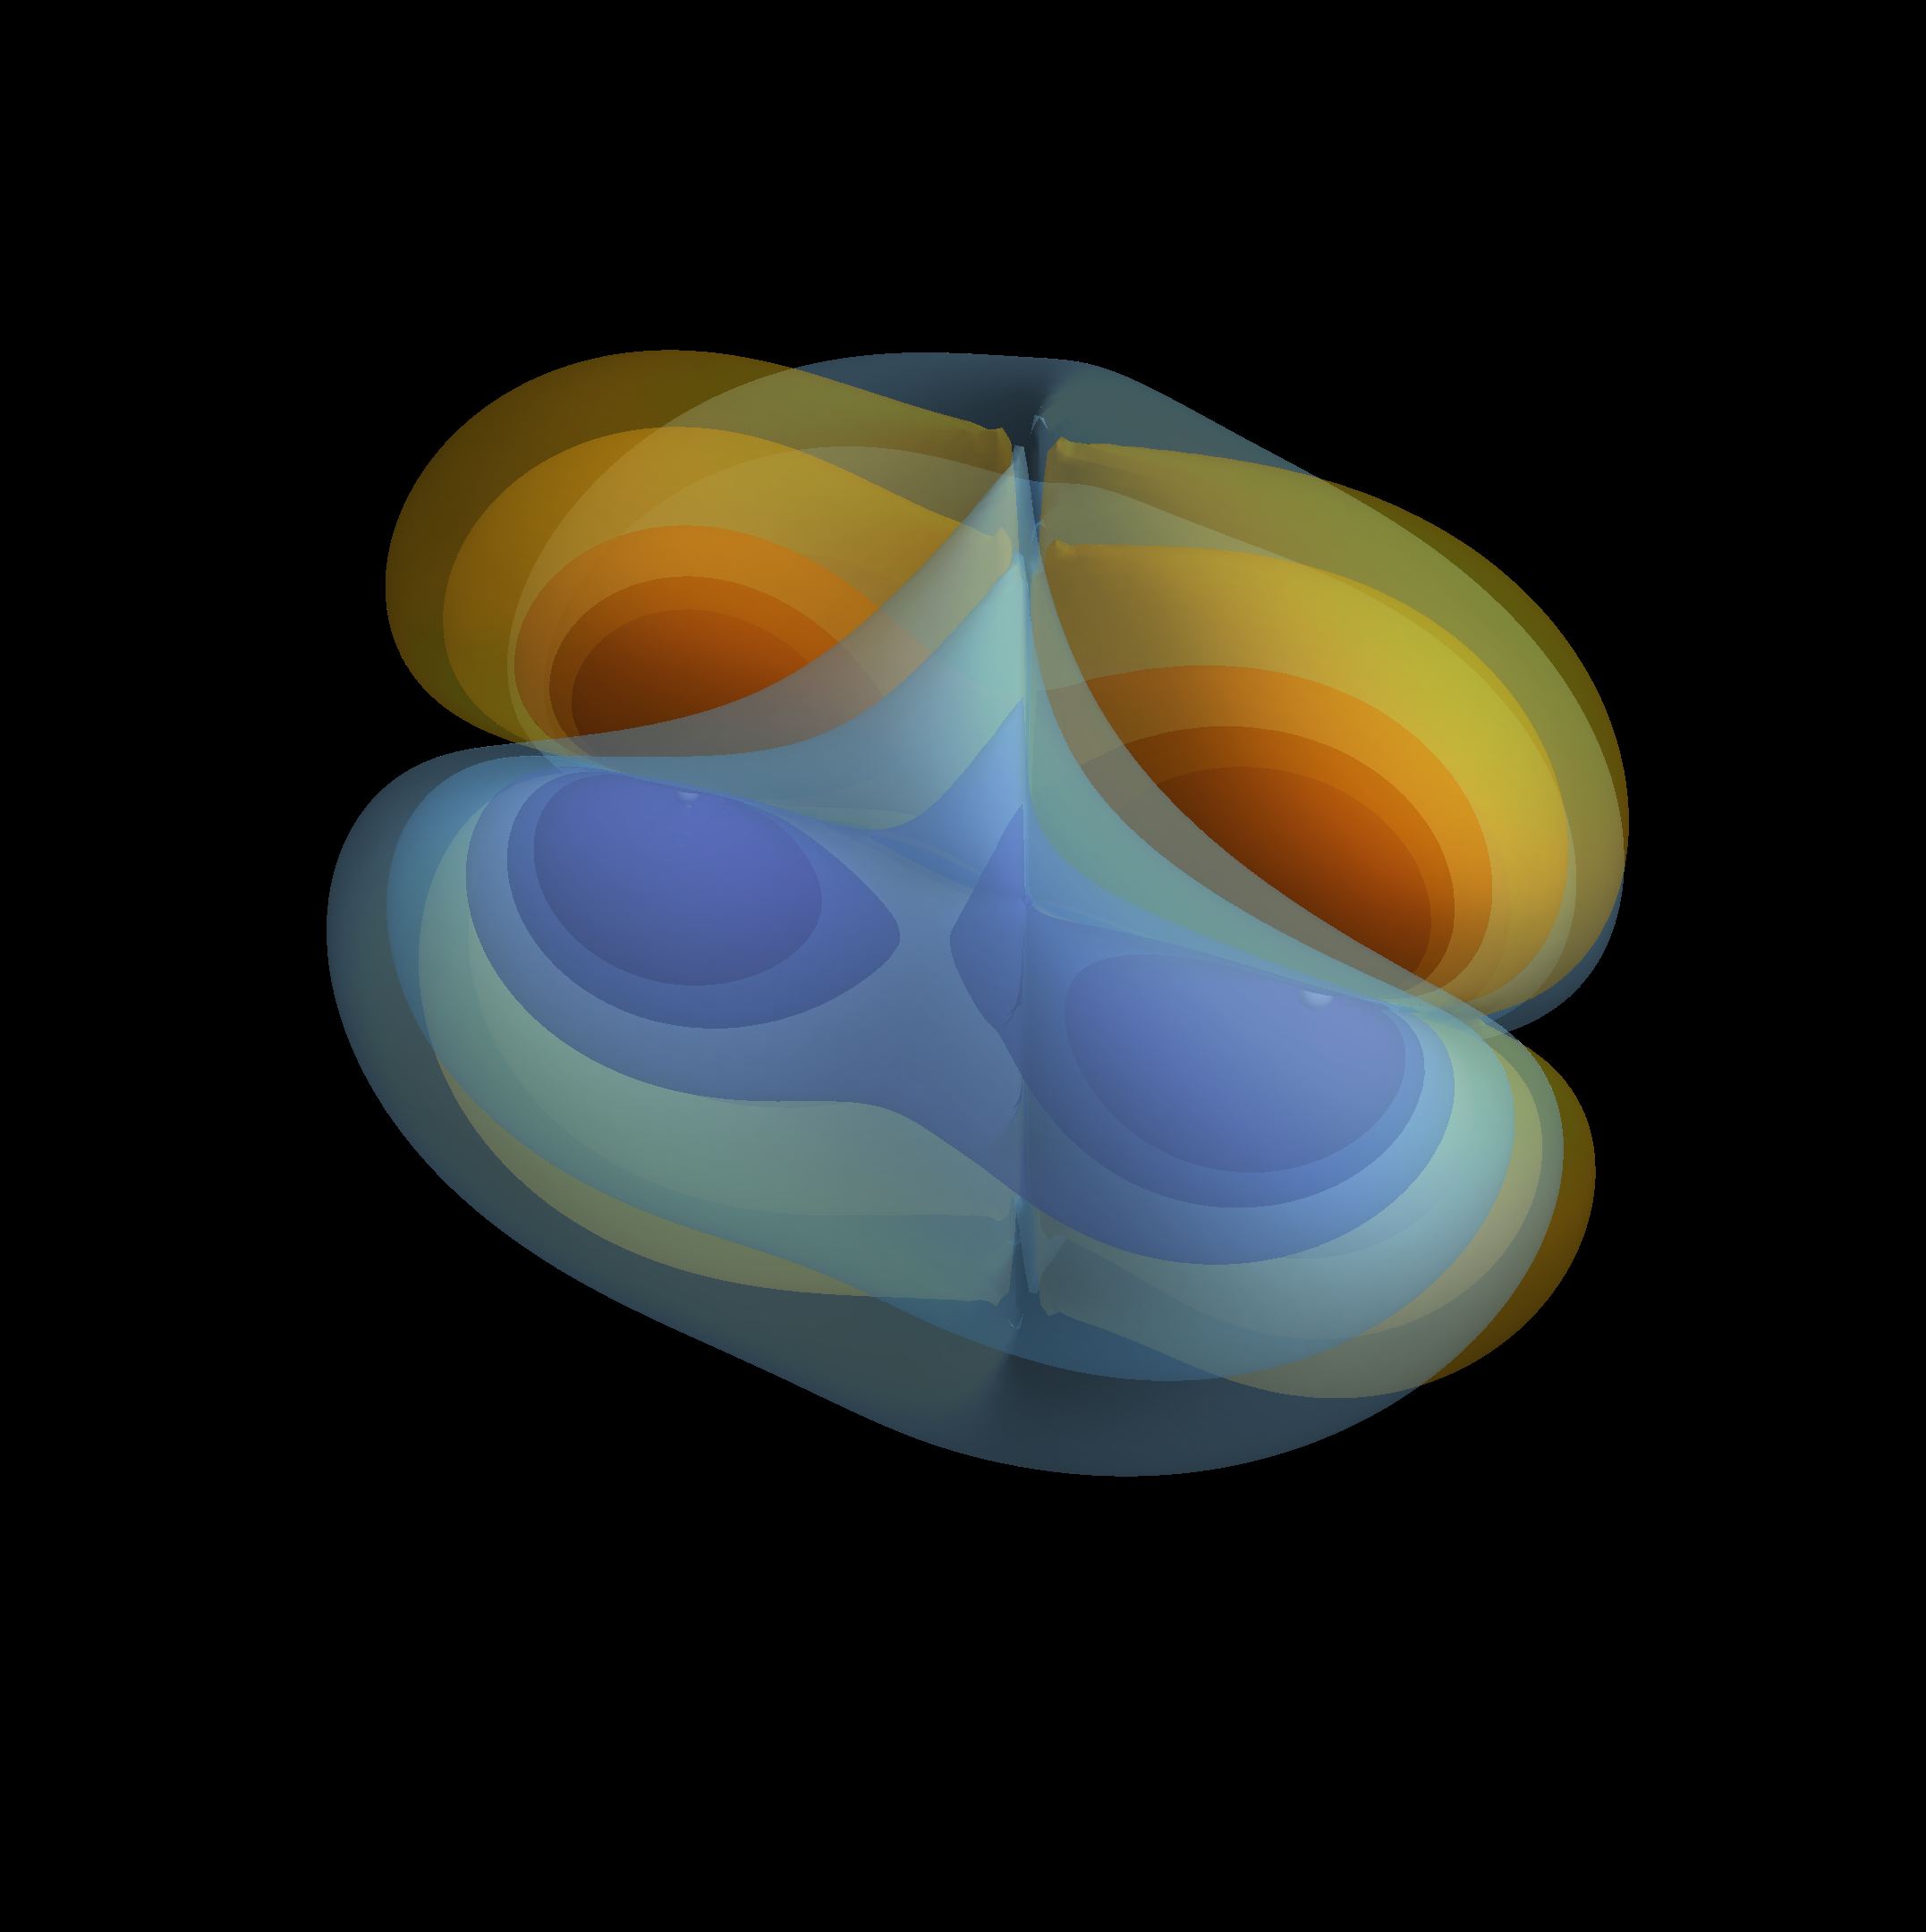
\includegraphics[scale=0.12]{Kap5/RePsi4.png}\caption{Real part of $\Psi_4$ representing outgoing gravitational radiation. Image taken from \textit{https://einsteintoolkit.org} \label{fig:psi4}}
\end{figure}
The importance of the Weyl scalar is seen in Figure \ref{fig:psi4}. This is a simulation of \textit{Einstein toolkit} code. Is made for a merger 36 + 29 solar mass binary black hole system. It is the $\Psi_4$ real part contribution of outgoing radiation in the wave zone. From this scalar we can characterize somehow the astrophysical systems and help to identify some aspects of them, for example, in gravitational collapse there is no gravitational radiation, this is because the Weyl tensor in this system is zero, therefore $\Psi_4=0$. For details see \cite{GRAVITATION}. 


